\chapter{Entwicklung der Atom- und Quantenphysik}

\section{Quantelung von Masse und Ladung}

\subsection{Quantelung der Masse}

\textbf{Chemie:}\\
Dalton'sches Gesetz der multiples Proportionen\\
Satz von Avogadro\\[5pt]
$ \Rightarrow $ Dalton'sche Atomhypothese\\
$ \Rightarrow $ Periodensystem der Elemente\\[5pt]
Periodizität festgestellt durch Atomvolumen. Erst später Ionisationsenergie (Abspaltung des am schwächsten gebundenen Elektron).\\[5pt]
\textbf{Physik:}\\
kinetische Gastheorie (vor allem Maxwell)\\
Gas $ = $ Teilchen mit nur kinetischer Energie, WW mit einem Gefäß
\begin{equation*}
\Rightarrow \quad P = \frac{N}{V} m \frac{\ol{v}^2}{3}
\end{equation*}
Äquipartitionstheorem
\begin{equation*}
\ol{E_{\tx{kin}}} = \frac{3}{2} k_B T \qquad (\tx{einatomiges Gas, } f = 3)
\end{equation*}
\begin{equation*}
\Rightarrow \quad \rmbox{P V = N_A k_B T} \qquad \tx{ideale Gas Gleichung}
\end{equation*}
$ V : $ Molvolumen\\
$ \Rightarrow $ Größe der Atome\\[5pt]
\emph{Beispiel:} \textbf{Messung der Gaskonstanten $ R $ über Schallgeschwindigkeit\\}
\begin{equation*}
c^2 = \frac{f + 2}{f} R \frac{T}{M} 
\end{equation*}
\folie{Versuchsaufbau zur Messung der Gaskonstante $ R $}

\subsubsection{Direkter Nachweis über die Rastertunnelmikroskopie}

Ein Elektron, das von einem in den anderen Energiezustand springt:
\begin{center}
	%t7:
	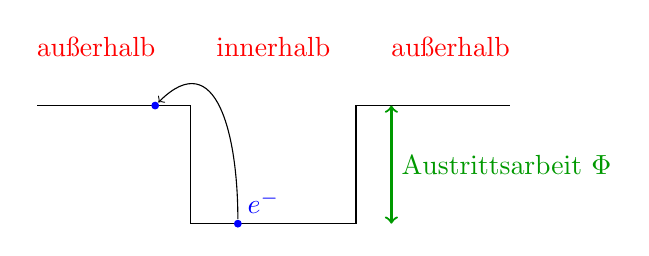
\begin{tikzpicture}[scale=.75]
		\draw (-4,0) -| (-1.4,-2) -- (1.4,-2) |- (4,0);
		\node[circle,fill=blue,inner sep=1pt,minimum size=1pt] (e) at (-.6,-2) {};
		\node[circle,fill=blue,inner sep=1pt,minimum size=1pt] (e2) at (-2,0) {};
		\draw[->,looseness=1.5] (e) to[out=90,in=45] (e2);
		\node[blue,anchor=south west] at (e) {$ e^- $};
		\draw[thick,black!40!green,<->] (2,0) -- node[right] {Austrittsarbeit $ \Phi $} (2,-2);
		\node[red] at (0,1) {innerhalb};
		\node[red] at (-3,1) {außerhalb};
		\node[red] at (3,1) {außerhalb};
	\end{tikzpicture}
\end{center}
\vspace{10pt}
Schematische Skizze eines Rastertunnelmikroskops:
\begin{center}
	%t8:
	\begin{tikzpicture}
		\coordinate (s) at (0,.5);
		% dreieck
		\draw[thick,pattern=north east lines,rounded corners=2pt] ($ (s) + (-.5,1.5) $) -- (s) -- ($ (s) + (.5,1.5) $);
		\coordinate (d) at (0,-1);
		% rechteck
		\draw[thick] ($ (d) + (-2,0) $) -- ($ (d) + (2,0) $);
		\draw[draw=none,pattern=north east lines] ($ (d) + (-2,0) $) -- ($ (d) + (2,0) $) [rounded corners=5pt] -- ($ (d) + (2,-.6) $) [rounded corners=5pt] -- ($ (d) + (-2,-.6) $) -- cycle;
		% bemaßung
		\draw[dashed] ($ (s) + (-1,0) $) -- ++(4,0);
		\draw[dashed] ($ (d) + (2,0) $) -- ++(1,0);
		\draw[red,thick,<->] ($ (s) + (-.5,0) $) -- node[left] {$ d $} ($ (d) + (-.5,0) $);
		% spannung
		\coordinate (U) at (-2.5,0);
		\draw[thick] ($ (U) + (-.2,0) $) -- ++(.4,0);
		\draw[thick] ($ (U) + (-.2,-.2) $) -- ++(.4,0);
		\draw[thick] (U) |- ($ (s) + (-.25,.75) $);
		\draw[thick] ($ (U) + (0,-.2) $) |- ($ (d) + (-2,-.3) $);
		\node[left] at ($ (U) + (-.2,-.1) $) {$ U $};
		% potential
		\coordinate (p) at ($ (s) + (3,0) $);
		\draw[thick] ($ (p) + (1,1) $) |- (p) -- ($ (d) + (3,0) $) -| ($ (d) + (4,-1) $);
		\draw[thick,black!40!green,<->] ($ (d) + (3,-.8) $) -- node[below] {$ \Phi $} ($ (d) + (4,-.8) $);
		% tunneling
		\coordinate (e1) at ($ (d) + (4,-.4) $);
		\coordinate (e2) at ($ (p) + (0,-.75) $);
		\coordinate (e3) at ($ (p) + (1,.4) $);
		\foreach \x in {e1,e2,e3}
		\node[circle,fill=blue,inner sep=1pt,minimum size=1pt] (\x) at (\x) {};
		\draw[blue,->,looseness=1.9] (e1) to[out=180,in=-140] (e2);
		\draw[blue,->,looseness=1.9] (e2) to[out=140,in=180] (e3);
		\draw[thick,->,red] (e1) to[out=120,in=-120] node[right] {Tunnelstrom} (e3);  
	\end{tikzpicture}
\end{center}
Der Tunnelstrom ist hierbei exponentiell zur Spannung proportional:
\begin{equation*}
I_T \propto U_T \tx{ exp}\left(- 2\sqrt{\frac{2 m \Phi}{\ol{k}^2}} d \right)
\end{equation*}
typische Zahlenwerte:\\
$ I_T $ ca. $ 1 - 10 \, \tx{mA} $\\
$ U_T $ ca. $ 100 \, \tx{mV} $\\
$ d $ ca. $ 1 - 10 \, \tx{nm} $\\
\folie{Rastertunnelmikroskop}\\
\lcom{Manövrieren mittels Piezokristallen um Präzisionen feiner als Atomare Skala zu erreichen.}\\
\folie{Rasterkraftmikroskop (AFM)}

% Vorlesung 11.12.18 (13 Days until christmas)

\subsection{Quantelung der Ladung}

\subsubsection{Elektrolyse}

\folie{zu Elektrolyse}\\
Prinzip $ \Rightarrow $ elektrische Ströme $ \Rightarrow $ Redox-Reaktion\\
$ \Rightarrow $ Stoffumsatz verknüpft mit Ladungsmenge
\begin{equation*}
F = e N_A = 96485{,}\dots \frac{\tx{C}}{\tx{mol}}
\end{equation*}
\emph{Beispiel:} NaCl
\begin{equation*}
2 Na^+ Cl^- \quad \rightarrow \quad 2 Na + Cl_2
\end{equation*}
Um 1 mal Na abzuscheiden, oder $ \frac{1}{2} $ mal Cl$ _2 $ Gas zu erzeugen werden $ Q = 96486 \, \tx{C} $ benötigt.
\begin{equation*}
\Rightarrow \quad F = N_A e \quad \Rightarrow e \approx 1{,}6 \cdot 10^{-19} \, \tx{C} 
\end{equation*}

\subsubsection{Millikan Versuch}

\folie{Milikan Versuch}\\
Prinzip: geladenes Tröpfchen + angelegtes $ \vec{E} $-Feld.
\begin{equation*}
\Rightarrow \quad m \vec{a} = q \vec{E} + m \vec{g} - \rho V \vec{g} + 6 \pi n R \vec{v}
\end{equation*}
\textbf{Schwebefeld-Methode}\\
Idee: $ \vec{E} $-Feld so einstellen, dass Tröpfchen schwebt.\\
Problem: $ R $ ist unbekannt.
\begin{equation*}
\Rightarrow \quad R \tx{ ungenau } \quad \Rightarrow \quad q \tx{ ungenau }
\end{equation*}
\versuch{Milikan Versuch}
Kondensator aus Gitterplatten und Seifenblasen als Tröpchen.\\[5pt]
\textbf{Gleichfeld-Methode}\\
Idee: Am selben Tröpfchen zwei Messungen mit unterschiedlichen $ \vec{E} $-Feldern.\\
Realisierung: $ \vec{E} $-Feld Umpolen\\[5pt]
Messung 1: Tröpfchen sinkt\\
Messung 2: Tröpfchen steigt\\
$ \Rightarrow R $ wird eliminiert
\begin{equation*}
v \tx{ messen } \Rightarrow \tx{ das geht ganz gut}
\end{equation*}
\folie{Millikan Ergebnisse}

\subsection{Bestimmung von \texorpdfstring{$ Q / M $}{Q/M} (Ladung/Masse)}

Prinzip:
\begin{enumerate}[1)]
	\item Teilchenstrahlquelle: geladene Teilchen werden durch $ \vec{E} $-Feld beschleunigt
	\item Massentrennung: Teilchenstrahl durch $ \vec{E} $- und $ \vec{B} $-Felder
	\item Teilchenstrahl detektieren
\end{enumerate}

\subsubsection{Teilchenstrahlquelle}

Glühkathode:
\folie{Glühkathoden}\\
Eine Drahtwindel wird in einem Vakuum stark erhitzt.\\
$ \Rightarrow $ Elektronen treten aus (überwinden Austrittsarbeit)
\begin{center}
	%t1:
	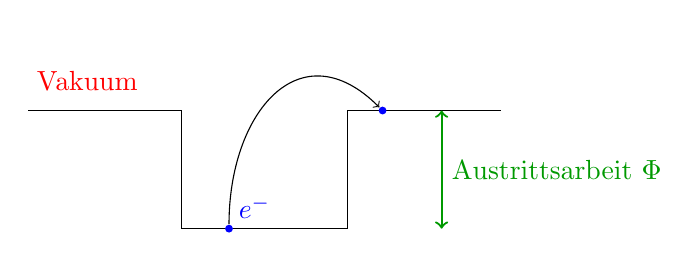
\begin{tikzpicture}[scale=.75]
		\draw (-4,0) -| (-1.4,-2) -- (1.4,-2) |- (4,0);
		\node[circle,fill=blue,inner sep=1pt,minimum size=1pt] (e) at (-.6,-2) {};
		\node[circle,fill=blue,inner sep=1pt,minimum size=1pt] (e2) at (2,0) {};
		\draw[->,looseness=1.5] (e) to[out=90,in=135] (e2);
		\node[blue,anchor=south west] at (e) {$ e^- $};
		\draw[thick,black!40!green,<->] (3,0) -- node[right] {Austrittsarbeit $ \Phi $} (3,-2);
		\node[red] at (-3,.5) {Vakuum};
	\end{tikzpicture}
\end{center}
$ \Rightarrow $ Elektronenstrahl durch Beschleunigungsspannung.

\subsubsection{Elektronenstoßionenquelle}

Atome/Moleküle werden mit Elektronen beschossen:
\begin{equation*}
A + e^- \rightarrow A^+ + 2 e^- \quad A^{++} + 3 e^-
\end{equation*}
\begin{equation*}
M + e^- \rightarrow M^+ + 2 e^- \quad M^{++} + 3 e^-
\end{equation*}
\emph{Beispiel: } $ H_2O + e^- \rightarrow H_2O^+, OH^+, O^+ \dots $\\
\folie{Elektronenstoßquelle}

\subsubsection{Elektrospray Ionenquelle (ESI)}

Prinzip: zu untersuchende Substanz wird in Flüssigkeit gebracht und mit dieser durch eine Düse aufgespritzt. Dabei wird außerdem eine hohe Spannung angelegt um die Tröpfchen zu beschleunigen.\\[5pt]
$ \Rightarrow $ Tröpfchen (1 - 10 nm)\\
$ \rightarrow $ Coulomb Explosion\\
$ \rightarrow $ Verdampfung der Flüssigkeit\\
\folie{Elektronenspray-Ionenquelle}

\subsubsection{Detektion}

\textbf{Faraday Becher}\\[5pt]
Gauß'scher Satz $ \Rightarrow $ Innerhalb um Metallkörper befinden sich keine Ladungen. Ladungen werden auf Außenseite gesammelt.\\[5pt]
Nachweisgrenze: $ 10^{-14} \, \tx{A} \ \widehat{=} \ 10^{5} \, \frac{\tx{Ionen}}{\tx{s}} $\\
\folie{Faraday-Becher}\\[5pt]
\textbf{Sekundärelektronenvervielfacher (SEV)}\\[5pt]
Ein auf Metall/Halbleiter auftreffendes Elektron erzeugt bei genügend Energie mehrere Sekundärelektronen.\\[5pt]
Nachweisgrenze: einzelnes Ion\\
\folie{SEV}\\
\folie{Mikrokanalplatte (für Ortsauflösung)}

\subsubsection{Massentrennung}

Teilchenstrahl durch $ \vec{E} $- und $ \vec{B} $-Felder\\
Magnetisches Feld:
\begin{equation*}
R = \frac{m}{q} \frac{v}{B}
\end{equation*}
Impulsfilter\\[5pt]
Elektrisches Feld:
\begin{equation*}
y(x) = \frac{q E}{2 m v_x^2} x^2
\end{equation*}
Energiefilter\\[5pt]
\folie{Magnetisches und elektrisches Feld}

\subsubsection{Thomson'sche Röhre}

\folie{Thomson'sche Röhre}\\
\folie{Massen-Spektren}\\
Beschleunigung:
\begin{equation*}
\frac{1}{2} m v^2 = q U
\end{equation*}
Ablenkung:
\begin{equation*}
m \frac{v^2}{R} = q v B
\end{equation*}
Für das Ladungs-Masse-Verhältnis ergibt sich dann.
\begin{equation*}
\Rightarrow \quad \frac{q}{m} = \frac{2 v}{(RB)^2}
\end{equation*}
\versuch{Glühkathode im Vakuum}
Der Elektronenstrahl wird sichtbar, da Argon-Moleküle im nicht perfekten Vakuum angeregt werden und blau leuchten. Durch das homogene Magnetfeld der Helmholzspulen wird aus dem Elektronenstrahl eine gekrümmte oder Kreisförmige Bahn. Bei Drehung des Glaskörpers ergibt sich eine Spirale.\\[5pt]
\versuch{Thomson'sche Röhre}
Prinzip wie beim Wien'scher Filter mit gekreuzten $ \vec{E} $- und $ \vec{B} $-Feldern.

\section{Struktur der Materie}

\subsection{Materie besteht aus Atomen/Ionen}

Dalton's Atomhypotese

\subsection{Atome bestehen aus Elektronen und ,,sonst etwas``}

$ \Rightarrow \quad e^- $ müssen gebunden sein\\
$ \Rightarrow $ Bindungsenergie für $ e^- $\\
$ \Rightarrow $ Ionisationsenergie: Bindungsenergie für ,,erstes`` Elektron $ e^- $

\subsubsection{Franck-Hertz-Versuch}

Idee:
\begin{enumerate}[1)]
	\item $ e^- $ werden im Atomgas beschleunigt, gewinne kinetische Energie. Je nach Wechselwirkung der $ e^- $ mit den Atomen tritt ein Energieverlust auf.
	\item Nach einer gewissen Strecke erreichte kinetische Energie wird gemessen
\end{enumerate}
Aufbau:
\folie{Franck-Hertz-Versuch}
\begin{itemize}
	\item Quecksilberdampf, ca. 10 mbar
	\item Glühkathode mit Beschleunigungsspannung
\end{itemize}

% Vorlesung 12.12.18 (12 Days until christmas)

\subsubsection{Photoionisation}

\versuch{Photoionisation}
Licht verschiedener Frequenzen wird auf Material gestrahlt. Bei bestimmter Frequenz wird viel absorbiert $ \Rightarrow $ Energie um äußerstes Elektron anzuregen.\\[5pt]
\folie{Photoionisation}\\
$ \Rightarrow $ direkte Bestimmung der Ionisationsenergie

\subsection{Atomkerne bestehen aus Atomschalen + Atomkernen}

\begin{equation*}
(e^-) \qquad \qquad \qquad (p,n)
\end{equation*}

\subsubsection{Rutherford-Experiment}

Idee:
\begin{enumerate}[1)]
	\item $ \alpha $ Teilchenstrahl $ \Rightarrow $ auf Gold-Folie geschossen
	\item Steuverteilung der $ \alpha $ Teilchen
\end{enumerate}
\folie{Rutherford-Experiment}\\
Coulombfelder (wie auch Gravitationsfelder) sind weitreichende Kräfte, da sie mit $ \frac{1}{r} $ abfallen. Ihr Beitrag ist auch bei sehr großen Entfernungen Messbar und nicht vernachlässigbar. Kräfte, die exponentiell oder schneller als mit $ \frac{1}{r} $ abfallen sind schnell abfallende Kräfte, die nicht weit reichen.\\
Um das Coulombpotential der Atomkerne zu überwinden und in ihre nähe zu gelangen benötigt man Strahlung mit viel Energie. Aufgrund der Feststellung, dass ein Großteil der Strahlung kaum gestreut wird können wir annehmen, die Atomkerne sind sehr klein. Bei dem Rutherford-Experiment liegt also Coulombstreuung vor.
\begin{itemize}
	\item fast nur Vorwärtsstreuung
	\item Streuung am Coulombpotential $ \Rightarrow $ kleine Kerne
\end{itemize}
\versuch{Rutherford-Experiment}
In Luft $ \Rightarrow $ keine $ \alpha $-Teilchen kommen am Detektor an. Im Vakuum ohne Goldfolie $ \Rightarrow $ ca. 650 - 740 Teilchen pro 10 s. Mit Goldfolie im Vakuum $ \Rightarrow $ ca 650 - 700 Teilchen pro 10 s. Bei Abgelenkten Teilchenstrahl und angewinkelter Goldfolie $ \Rightarrow $ gelegentlich ein par gestreute Teilchen im Detektor.\\
\folie{Atommodell}\\
\textbf{Verhältnis von Atomkern zu Elektronenhülle:} $ 10^{-4} = \frac{1}{10000} $ mal Kleiner.

\subsection{Festkörper bestehen aus einer periodischen Anordnung von Atomen}

Dies kann man mit der \textbf{Bragg-Streuung} zeigen.\\[5pt]
Bei Röntgenstrahlung (X-ray) messen wir die Streuung an der Elektronenhülle ($ \vec{F} = q \vec{E} $). Wir messen die Ladungsdichte der Elektronen.\\
Bei Neutrinos: nichts (sie wechselwirken kaum mit Materie)\\
Bei Elektronen: Streuung an Elektronenhülle. Starkes $ \vec{E} $-Feld $ \rightarrow $ kleine Eindringtiefe $ \rightarrow $ Oberflächenmessung.\\
Alphateilchen sind erstens sehr massiv und positiv geladen und wechselwirken daher mit den Kernen und gehen durch die Elektronenhülle durch.\\
Bei Neutronen: Streuung am Kern: starke WW (WW zwischen Kernbausteinen) ,,Kernkraft``. Messung der Kernpositionen.\\

\section{Quantelung von Energie, Planck'sches Strahlungsgesetz}

\subsection{Energiezustände, Spektren}

\begin{minipage}{.6\linewidth}
	\textbf{diskrete Spektren sind diskreten (gequantelten) Energiezuständen zugewiesen}\\
	Energiezustände werden auch manchmal Spektren genannt Energiespektrum $ \neq $ Spektrum \\(Energie-Differenzen)
\end{minipage}%
\begin{minipage}{.4\linewidth}
	\flushright
	%t1:
	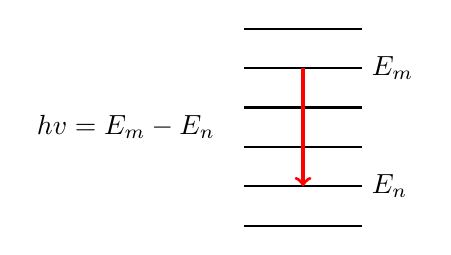
\begin{tikzpicture}
		\foreach \c in {.5,1,1.5,2,2.5,3}
		\draw[thick] (1,\c) -- (2.5,\c);
		\draw[red, very thick, ->](1.75,2.5) -- (1.75,1);
		\node at (-0.5,1.75) {$hv=E_m-E_n$};
		\node[right] at (2.5,1) {$ E_n $};
		\node[right] at (2.5,2.5) {$ E_m $};
	\end{tikzpicture}
\end{minipage}%

\subsubsection{Quantenmechanische Beschreibung}

\begin{itemize}
	\item \textbf{Zustände:} $ |\psi \rangle $\\
	Bei Koordinatentransformationen verändern sich die Koordinaten, Vektoren bleiben gleich. Für die Angabe von Koordinaten benötigt man eine Basis oder einen Ursprung.\\
	Genauso braucht man für Wellenfunktionen eine Basis. Für Zustände nicht (sie repräsentieren im Beispiel hier die Vektoren). \textbf{(Lage der Peaks)}
	\item \textbf{Übergänge zwischen den Zuständen} $ \langle \psi | \hat{V} | \psi'\rangle $\\
	Der \textbf{Operator} $ \hat{V} $ ist die Wechselwirkung. Der Operator eines Neutrinos wäre also $ = 0 $ (Bzw. die Übergangselement-Matrix ist $ = 0 $). Bei X-rays wäre der Operator der Dipoloperator, da die positiven X-rays mit den Elektronen wir ein Dipol Wechselwirken. \textbf{(Intensität der Peaks)}\\
	Definiert man einen Zustand als Vektor $ \vec{v} $ so ist der Übergang dann $ \vec{v}^\top \overset{\circ}{A}\ \vec{v} $
	\item Ensemble von Objekten $ \leftrightarrow $ Besetzungszahlen (-wahrscheinlichkeiten) \\
	Beim thermodynamischen Gleichgewicht:
	\begin{equation*}
	n_i \propto e^{- \beta E_i} \quad \beta = \frac{1}{k_B T}
	\end{equation*}
\end{itemize}
\versuch{Spektren mit Leuchtstoffröhren}
Helium Gas: Spektrum mit diskreten Linien\\
Neon Gas: Weniger diskrete Maxima und eher höhere Frequenzen\\
anderes Gas: Türkis (andere Frequenzen zu hoch für menschliches Auge)\\
Wasserstoff: wenige diskrete Peaks

\subsubsection{Balmer-Serie des Wasserstoffs}

\begin{equation*}
f = R_y\left(\frac{1}{n^2} - \frac{1}{m^2}\right) \qquad R_y = 13{,}6 \, \tx{eV}
\end{equation*}

% Vorlesung 18.12.18 (6 Days until christmas)

\subsection{Hohlraumstrahlung}

Strahlung eines K"orpers mit Temperatur $T$ genauer:\\[5pt]
Strahlung eines K"orpers im thermodynamischen Gleichgewicht mit Strahlungsfeld.\\[5pt]
\textbf{Schwarzer K"orper}\\
Strahlung jeder Wellenl"ange wird vollst"andig absorbiert.\\
thermodynamisches GGW $\Leftrightarrow$ K"orper strahlt im gleichen Maße ab wie er auch absorbiert (für jede Frequenz !). \\[5pt]
\textbf{Hohlraumstrahler}\\
Strahlung jeder Wellenl"ange wird vollst"andig absorbiert. Emission jedoch nicht von ganzen K"orper, sondern nur einem kleinen Loch.\\[5pt]
Gesucht $ \Rightarrow $ Intensität als Funktion der Frequenz:
\begin{itemize}
	\item Energiedichte der Strahlung $ \omega(f) $ oder Energie im Frequenzintervall $ \omega(f) \, \dd f $
\end{itemize}

\subsubsection{Grundlage der Beschreibung von Hohlraumstrahlung}

\begin{minipage}{.6\linewidth}
	\begin{enumerate}[$ \Rightarrow $]
		\item Randbedingungen für EM-Wellen
		\item Frequenz/Wellenlängen sind eingeschränkt
		\item Moden
		\item Modendichte $ g(f) $
		\begin{equation*}
		g(f) \dd f = \frac{ 8 \pi f^2 }{c^3} \dd f
		\end{equation*}
	\end{enumerate}
\end{minipage}%
\begin{minipage}{.4\linewidth}
	\flushright
	%t1:
	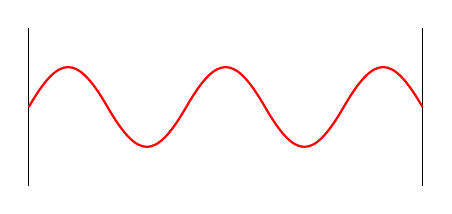
\begin{tikzpicture}
		\draw (0,0) -- (0,2);
		\coordinate (a) at (5,0);
		\draw (a) -- ++(0,2);
		% \draw[decorate,decoration={snake,amplitude = .5cm}] (0,1) -- ($ (a) + (0,1) $);
		\draw[thick,red,looseness=2] (0,1) to[out=60,in=120] (1,1) to[out=-60,in=-120] (2,1) to[out=60,in=120] (3,1) to[out=-60,in=-120] (4,1) to[out=60,in=120] (5,1);
	\end{tikzpicture}
\end{minipage}%
\begin{enumerate}[$ \Rightarrow $]
	\item Energiedichte $ w(f) $
	\begin{equation*}
	w(f,T) \dd f = g(f) \ol{W}(f,T) \dd f
	\end{equation*}
	$ \ol{W}(f,T) : $ mittlere Energie pro Mode im Frequenzintervall $ \dd f $
\end{enumerate}

\subsection{Klassische Berechnung: Rayleigh-Jeans Gesetz}

Thermodynamisches GGW: Äquipartitionstheorem $ f = 2 $ (Die ebene der Polarisationsrichtungen einer EM-Welle)\\[5pt]
$ \Rightarrow \ol{W} = k T $
\begin{equation*}
\Rightarrow \rmbox{w(f,T) = \frac{8 \pi f^2}{c^3} k T}
\end{equation*}
\lcom{Bei diesem Ergebnis gibt es das Problem, dass die Energiedichte für sehr große Frequenzen gegen unendlich geht. \lightning}\\
Problem:
\begin{itemize}
	\item $ f \to \infty \Rightarrow $ UV-Katastrophe
	\item Stimmt nicht mit Experiment überein. (Nur für kleine Frequenzen!)
\end{itemize}

\subsection{Planck'sches Strahlungsgesetz I}

Annahme für die Energie einer Mode:
\begin{equation*}
W_n = n h f \qquad n = 0,1,2, \dots \infty
\end{equation*}
$ n : $ Besetzungszahl der Mode\\[5pt]
$ \Rightarrow $ Besetzungszahldichte im thermodynamischen GGW:
\begin{equation*}
p_n = \frac{e^{-\frac{w_n}{kT}}}{Z(T)} = \frac{e^{-\frac{n h f}{k T}}}{\sum_n e^{-\frac{nhf}{kT}}}
\end{equation*}
$ \Rightarrow \quad \ol{W} = \sum_n p_n w_n $\\[5pt]
$ \Rightarrow \quad \ol{W} = \frac{hf}{e^{\frac{hf}{kT}} - 1} $
\frbox{Plank'sches Strahlungsgesetz}{
\begin{equation*}
\Rightarrow \quad w(f) = \frac{8 \pi h f^3}{c^3} \frac{1}{e^{\frac{hf}{kT}} - 1}
\end{equation*}}
\noindent
\folie{Plank'sches Strahlungsgesetz}

\subsubsection{Wien'sches Verschiebungsgesetz}

$$ f_{\tx{max}} \propto T $$
\emph{Bemerkung:}
\begin{equation*}
\lambda_{\tx{max}} \neq \frac{c}{f_{\tx{max}}} \ \ \color{red} \tx{\mau} \color{black}
\end{equation*}

\subsubsection{Stefan-Boltzmann Gesetz}

$$ P \propto T^4 $$
$ P : $ gesamte Strahlungsleitung\\[10pt]
\versuch{Spektrum einer Glühlampe}
\emph{Beispiel:} \textbf{Sonne}\\[5pt]
\folie{Strahlungsspektrum der Sonne (aus dem Weltall)}\\
Stefan Boltzmann $ \Rightarrow T_{\tx{Sonnenoberfläche}} \approx 5777 \, \tx{K} $\\
Wien $ \quad \ \: \qquad \qquad \Rightarrow T_{\tx{Sonnenoberfläche}} \approx 5800 \, \tx{K} $\\
$ \Rightarrow $ Das Modell ,,Sonne = schwarzer Körper`` stimmt ungefähr aber nicht perfekt.

\subsection{Gedanken zum Plank'schen Strahlungsgesetz}

Grenzfälle:
\begin{itemize}
	\item $ \frac{hf}{kT} \to 0 : $ $ \ol{W} \to kT \Rightarrow $ Rayleigh Jeans $ \widehat{=} $ klassischer Fall
	\item $ \frac{hf}{kT} \to \infty : $ $ \ol{W} \to (hf)^3 e^{-\frac{hf}{kT}} \Rightarrow $ keine UV-Katastrophe $ \widehat{=} $ quantenmechanischer Grenzfall
\end{itemize}
$ \Rightarrow $ Das Gesetz impliziert \textbf{Quantum für Licht (Photon)}
\begin{equation*}
\rmbox{E = hf = \hbar \omega }
\end{equation*}
Energiespektrum einer Schwingungsmode.\\
\begin{minipage}{.6\linewidth}
	Wie ist die Quantisierung der kontinuierlichen Kurve zu sehen?\\
	Aus dem exponentiellen Abfall des Kurve bei niedrigen Wellenlängen mit $ e^{-\frac{hf}{kT}} $ sehen wir es muss ein $ hf > 0 $ geben. Dies ist der in rot eingezeichnete erste Energiesprung vom untersten, ins erst höhere, Niveau.
\end{minipage}%
\begin{minipage}{.4\linewidth}
	\flushright
	%t2:
	\begin{tikzpicture}
		\draw[thick,->] (0,.4) -- (0,4.6);
		\foreach \y in {.8,1.6,2.4,3.2,4}
		\draw[thick] (.5,\y) -- ++(3,0);
		\draw[thick,red,<->] ($ (.5,.8) + (1.5,0) $) -- node[right] {$ \hbar \omega $} ($ (.5,1.6) + (1.5,0) $);
		\foreach \y\l in {.8/1,1.6/3,2.4/5,3.2/7,4/9}
		\node[right] at ($ (.5,\y) + (3,0) $) {$\frac{\l}{2} \hbar \omega $};
	\end{tikzpicture}
\end{minipage}%
\\
\begin{equation*}
\frac{hf}{kT} \to \infty \quad \Leftrightarrow \quad w(f) \propto e^{-\frac{hf}{kT}}
\end{equation*}
Besetzungszahlen
\begin{itemize}
	\item klassisch $ \qquad \qquad \quad \frac{hf}{kT} \to 0  \Rightarrow $ alle Zustände nahezu gleich besetzt $ P_n \approx \frac{1}{N} $
	\item quanten mechanik $ \ \ \ \, \, \frac{hf}{kT} \to \infty \Rightarrow $ alle Zustände exp. schwach besetzt bis auf Grundzustand\\
	$ P_0 \approx 1 \quad P_1 \approx e^{-\frac{hf}{kT}} \quad P_n \propto e^{- n \frac{hf}{kT}} $
\end{itemize}
\emph{Beispiel:} \textbf{Einstein Modell für spezifische Wärme in Festkörpern}\\[5pt]
klassisch: Äquipartitionstheorem $ c_v = 3 N K $
\begin{equation*}
\ol{W} = \frac{6}{2} k T = 3 kT \qquad U = N \ol{W}
\end{equation*}
\begin{equation*}
c_v = \prt{U}{T}\bigg|_V = 3 N k
\end{equation*}
Einstein Modell: alle Gitterschwingungen schwingen mit Frequenz $ f_0 $.
\begin{equation*}
\Rightarrow \quad W_n = n k f_0 = n \hbar \omega_0
\end{equation*}
\begin{equation*}
\Rightarrow \quad c_v = 3 N k \left(\frac{\hbar \omega_0}{kT}\right)^2 \frac{e^{\frac{\hbar \omega_0}{kT}}}{\left[e^{\frac{\hbar \omega_0}{kT}} - 1\right]^2}
\end{equation*}
\folie{Einstein Modell: Plot  von $ c_v $}\\
$ \Rightarrow \quad c_v(T \to 0) \propto e^{-\frac{\hbar \omega_0}{kT}} \quad \Leftrightarrow \quad  $ System ,,friert`` aus.

% Vorlesung 19.12.18 (5 Days until christmas)

\noindent
\folie{Energie einer EM-Welle quadratisch von der Amplitude (wie Intensität von der Feldstärke)}

\subsection{Plank'sches Strahlungsgesetz II: Einstein}

\folie{Energieniveaus und 3 Prozesse:}\\
spontane Emission, Absorption und stimulierte Emission.\\[5pt]
Ensemble von Objekten
\begin{equation*}
\prd{N_2}{t} = - \prd{N_2}{t} \bigg|_{\tx{spont. Emission}} + \prd{N_2}{t} \bigg|_{\tx{Abs.}} - \prd{N_2}{t} \bigg|_{\tx{stim. Emission}}
\end{equation*}
$ \dot{N}_1 $ Analog dazu\\[5pt]
\textbf{Thermodynamisches Gleichgewicht:}
\begin{enumerate}[i)]
	\item Boltzmann.Faktor
	\begin{equation*}
	\frac{N_2}{N_1} = \frac{e^{-\frac{E_2}{kT}}}{e^{-\frac{E_1}{kT}}} = e^{-\frac{E_2 - E_1}{kT}}
	\end{equation*}
	\item $ E_2 - E_1 = h f $
	\item stationär
	\begin{equation*}
	\dot{N}_2 \big|_{\tx{Abs.}} = \dot{N}_2 \big|_{\tx{spont. Emission}} + \dot{N}_2 \big|_{\tx{stim. Emission}}
	\end{equation*}
	\item 
	
	% make align nicer
	
	\noindent
	\begin{align*}
	\dot{N}_2 & \big|_{\tx{Abs.}} \qquad \quad \ \ \, = B \sigma(f) N_1\\
	\dot{N}_2 & \big|_{\tx{stim. Emission}} \ = C \sigma(f) N_2\\
	\dot{N}_2 & \big|_{\tx{spont. Emission}} = A N_2
	\end{align*}
	$ \sigma(1) : $ Energiedichte des Strahlungsfelds\\[5pt]
	Im thermodynamischen Gleichgewicht: $ \sigma(f) = w(f) $
	\begin{equation*}
	\Rightarrow \quad B w(f) N_1 = A N_2 + C w(f) N_2
	\end{equation*}
	\begin{equation*}
	\Rightarrow \quad w(f) = \frac{A}{B e^{\frac{hf}{kT}} - C}
	\end{equation*}
	\item klassischer Grenzfall $ T \to \infty $:
	\begin{equation*}
	\Rightarrow \quad B = C \qquad \Rightarrow \quad w(f) = \frac{A}{B} \frac{1}{e^{\frac{hf}{kT}} - 1}
	\end{equation*}
	\item Vergleich mit Rayleigh-Jeans:
	\begin{equation*}
	\Rightarrow \quad \frac{A}{B} = \frac{8 \pi f^2}{c^3} h f
	\end{equation*}
\end{enumerate}
\textbf{Konsequenzen}
\begin{enumerate}[1)]
		\item
		\begin{equation*}
		w(f) = \frac{8 \pi h f^3}{c^3} \frac{1}{e^{\frac{hf}{kT}}-1}
		\end{equation*}
		\item drei Prozesse
		\item $ \frac{A}{B} = \frac{8 \pi h f^3}{c^3} $
		\item MASER (M $ \widehat{=} $ Mikrowellen), später LASER
\end{enumerate}

\section{Welle-Teilchen Dualismus}

\subsection{Photoelektrischer Effekt (Photoeffekt)}
\folie{äußerer Photoeffekt, Hallwachs Versuch}\\
Photoeffekt:\\
Wechselwirkung mit Licht führt zu Absorption eines Photons und Emission eines Elektrons.
\begin{enumerate}[i)]
	\item äußerer Photoeffekt
	\item innerer Photoeffekt in Halbleitern
	\item Photoionisation
\end{enumerate}
\versuch{Halwachs Versuch}
Aufbau:\\
UV-Lampe (Viel UV aber auch sichtbares Weißes Licht), die über Kollimatorlinse und eine Lochblende auf Zinkplatte strahlt. Daran angeschlossen ist ein Elektrometer.
\begin{enumerate}[i)]
	\item Die Zinkplatte wird negativ aufgeladen. Wird die Abdeckung weggenommen so nimmt die Ladung auf der Platte schnell ab. Die Elektronen werden also aus dem Material ausgestoßen.
	\item Die Zinkplatte wird positiv aufgeladen. Wird die Abdekung nun weggenommen passiert nichts. Die Ladung bleibt auf der Platte.
	\item Die Zinkplatte wird wieder negativ aufgeladen. Die Abdeckung wird mit einer Glasplatte ersetzt so tut sich nichts oder nur sehr wenig. Wird die Glassplatte entfernt passiert das selbe wir bei i).
	\item Tageslicht funktioniert nicht oder nur sehr langsam.
\end{enumerate}
\textbf{Interpretation:}
\begin{enumerate}[i)]
	\item freigesetzte $ e^- $ werden von Ladung auf der Platte abgestoßen\\
	$ \Rightarrow $ Ladung sinkt ab
	\item freigesetzte $ e^- $ werden von Ladung auf der Platte angezogen\\
	$ \Rightarrow $ Ladung bleibt gleich
	\item kaum UV-Strahlung $ \Rightarrow $ nichts $ \Rightarrow $ Effekt hängt von $ f $ ab nicht von der Intensität
	\item Tageslicht reicht nicht um $ e^- $ herauszuschlagen
\end{enumerate}
\rbox{$ \Rightarrow $ Effekt hängt von $ f $ ab, nicht von der Intensität.}
\versuch{Leonard Versuch (Theorie)}
\folie{Versuchsaufbau}\\
Die Energie der Elektronen ist begrenzt durch die hineingesteckte Energie minus die Austrittsenergie.\\[5pt]
Aufbau (Gegenfeldmethode: anders herum als auf der Folie abgebildet):
\begin{itemize}
	\item Photokathode wird mit Licht bestrahlt
	\item freigesetzte $ e^- $ werden durch ein elektrisches Gegenfeld einer Anode abgebremst
	\item Die Anzahl der hier noch durchkommenden Elektronen wird als Photostrom gemessen
\end{itemize}
\emph{Bemerkung:}
\begin{itemize}
	\item freigesetzte $ e^- $ haben kinetische Energie mit einer (unbekannten) Verteilung. Mit Gegenspannung $ U $ wird die maximale kinetische Energie bestimmt: $ U_0 \Leftrightarrow I_{\tx{Photo}} = 0 $
\end{itemize}
\textbf{Beobachtung:}\\
\folie{Graph der Energie gegenüber der Frequenz des eingestrahlten Lichts}
\begin{enumerate}[i)]
	\item $ U_0 = \const \cdot f - \frac{W_A}{e} $
	\item Der Photostrom ist proportional zur Intensität des Lichts.
	\item Die Gegenspannung $ U_0 $ hängt \textbf{NICHT} von der Intensität ab.
	\item Es gibt eine minimale Spannung $ \frac{W_A}{e} $
	\item Achsenabschnitt bzw. Wert von $ \frac{W_A}{e} $ ist materialabhängig (die Steigung jedoch nicht)
\end{enumerate}
\begin{minipage}{.55\linewidth}
	\textbf{Interpretation:}\\
	Energie des Lichts wird an $ e^- $ in Metall abgegeben\\
	$ \Rightarrow $ $ e^- $ treten mit maximaler kinetischer Energie aus:
\end{minipage}%
\begin{minipage}{.45\linewidth}
	%T Tikz mit austrisstarbeit eines elektrons:
	%t1:
	\flushright
	\begin{tikzpicture}[scale=.75]
		\draw (-4,0) -| (-1.4,-1.5) -- (1.4,-1.5) |- (4,0);
		\node[circle,fill=blue,inner sep=1pt,minimum size=1pt] (e) at (-.6,-1.5) {};
		\node[circle,fill=blue,inner sep=1pt,minimum size=1pt] (e2) at (2,0) {};
		\draw[->,looseness=1.5] (e) to[out=90,in=135] (e2);
		\node[blue,anchor=south west] at (e) {$ e^- $};
		\draw[thick,red,<->] (3,0) -- node[right] {$ W_A $} (3,-1.5);
	\end{tikzpicture}
\end{minipage}%
\\
$ \Rightarrow \quad e U = E_{\tx{Licht}} - W_A $\\[5pt]
$ \Rightarrow $ Experiment: $ E_{\tx{Licht}} = h f $\\[5pt]
Entscheidend: klassisch:
\begin{equation*}
W = \frac{1}{2} \epsilon_0 (E^2 + c^2 B^2) = \frac{1}{c} I
\end{equation*}

\subsubsection{Einstein's Photonenhypothese}

Licht verhält sich wie ein Teilchenstrom. Diese Teilchen nennen wir Photonen. Sie haben eine Energie von $ E = h f $
\begin{equation*}
\Rightarrow \quad \rmbox{e U = h f - W_A}
\end{equation*}
$ \Rightarrow $ Nobelpreis 1921

\section*{Fragerunde}

\addcontentsline{toc}{section}{V. \texorpdfstring{\ \ \: }{space}  Fragerunde}

\textbf{Zu Leonard Versuch: Warum das Magnetfeld:}\\
Nur Teilchen mit bestimmter Masse (Elektronenmasse) kommen in den Detektor, nicht auch andere Teilchen, die irgendwie anders in dieselbe Richtung fliegen. (Glaßkörper ist nicht perfekt ...).\\[5pt]

% Vorlesung 8.01.19

\noindent
\versuch{Leonard Versuch (Praktisch)}
\begin{enumerate}[i)]
	\item
	\begin{equation*}
	U_{\tx{max}} = \const \cdot f - U_0 \quad U_0 = \frac{W_A}{e}
	\end{equation*}
	\item Photostrom $ \propto $ Intensität des einfallenden Lichts.
	\item Die Gegenspannung ist von der Intensität unabhängig.\\
	\lcom{Hier scheitert die klassische Interpretation. Nehmen wir an die Energie des Lichts sei an die Intensität gebunden so würden wir erwarten, bei höherer Energie eine höhere Gegenspannung zu messen. Dies ist aber nicht so. Die Energie die auf ein Elektron übertragen wird ist $ E = h f $ also die Energie eines Photons und damit Frequenzabhängig nicht Intensitätsabhängig. Die Intensität sorgt nur für mehr Elektronen pro Zeiteinheit aber nicht für Elektronen mit mehr Energie.}\\
	$ \Rightarrow $ Einstein:
	\begin{equation*}
	E_{\tx{Photon}} = hf
	\end{equation*}
\end{enumerate}
\begin{center}
	%t1:
	\begin{tikzpicture}
	\draw[->] (0,-2) -- (0,3) node[anchor=south east] {Spannung $ U $ in V };
	\draw[->] (-.2,0) -- (6,0) node[anchor=north west] {Frequenz $ f $};
	\foreach \y\x in {0/1.5, 0.8/3, 1/3.5, 2/4.5, 2.4/5}
	\draw ($ (\x,\y) - (.1,.1) $) -- ++(.2,.2) ($ (\x,\y) + (-.1,.1) $) -- ++(.2,-.2);
	\draw (-.5,-2) -- ++(38:8);
	\foreach \y\x\l in {0/1.5/ , 0.8/3/ , 1/3.5/grün, 2/4.5/blau, 2.4/5/ }
	\draw ($ (\x,0) + (0,.1) $) -- ++(0,-.2) node[below] {\l} ($ (0,\y) + (.1,0) $) -- ++(-.2,0);
	\foreach \y\v in {.5/0{,}4, 1.2/0{,}5, 2/1{,}0, 2.6/1{,}2}
	\node[left] at (0,\y) {\v V};
	\node[above] at (1.5,.1) {rot};
	%\draw[decorate, decoration={brace,amplitude=10pt,raise=2pt}, xshift=2pt,scale=.1]  (0,-10.2) -- node[anchor=south east, xshift=-15pt, yshift=15pt] {$\lambda = \frac{2 \pi}{k}$}  (0,0);
	\node[yscale=2.2, xscale=1.25,rotate=-90] at (-.15,-.8) {$ \ub{} $};
	\node[left] at (-.3,-.7) {$ W_A $};
	\end{tikzpicture}
\end{center}

\subsection{Anwendungen des Photoeffekts}

%T1

\begin{equation*}
U_{\tx{max}} = \const \cdot f - U_0 \quad U_0 = \frac{W_A}{e}
\end{equation*}
PES: Photoelektronenspektroskopie\\[5pt]
Material mit Licht bestrahlen $ \Rightarrow $ auustretende Photoelektronen genau analysieren.\\
$ \Rightarrow $ Materialanalyse
\begin{itemize}
	\item[$ e^-: $] geringe Eindringtiefe von wenigen hundert Angström, kurze Weglängen $ \Rightarrow $ Oberflächen, Filme, ...
\end{itemize}
UPS: UV Licht\\
(typische Enegie Licht: $ 1-2 \tx{eV} $ wie oben im Diagramm zu sehen,
typische Energie Röntgen: $ 10-100 \tx{keV} $,
typische Energie Radioaktivität: mehrere MeV.)\\
$ \Rightarrow $ Spektroskopie an Valenzelektronen.\\[5pt]
XPS: X-ray Strahlung\\
$ \Rightarrow $ Spektroskopie an Core-Elektronen (innere Schalen)\\
$ \Rightarrow $ Elementanalyse\\

\subsubsection{Photomultiplikator}

\folie{Photomultiplikator}\\
\textbf{Zum Teilchenbild}\\
\folie{Harmonischer Oszillator und Potential und Äquidistantes Energiespektrum}\\
Die Energien der Zustände sind im Potential des harmonischen Oszillators \textbf{Äquidistant}.

\subsection{Compton-Effekt (Licht verhält sich wie Teilchen)}

\folie{Compton-Effekt}\\zerfall
Streuung eines Photons an einem nominell freien Elektron.
\hfw (lambda oder R)
\begin{equation*}
\lambda_S = \lambda_0 + 2 \lambda_c \sin^2 \left(\frac{\theta}{2}\right)
\end{equation*}
\begin{equation*}
\lambda_c = \frac{k}{m_0c} \approx 2{,}4 \tx{pm}
\end{equation*}
Beobachtung für weißes Licht\\[5pt]
\versuch{Compton-Effekt}
$ \Rightarrow $ es zeigt sich, dass sich Licht in ,,allen`` (vielen kinematischen) Aspekten wie ein Teilchen verhält.
\begin{align*}
E &= hf\\
\vec{p} &= \hbar \vec{k} \qquad k = \frac{2 \pi}{\lambda}
\end{align*}
Dispersionsrelation:
\begin{equation*}
\rmbox{E(\vec{p}) = cp} \quad (\tx{masseloses/relativistisches Teilchen})
\end{equation*}

\subsection{Teilchenstrahl Beugung/Interferenz (Teilchen verhalten sich wie Wellen)}

Doppelspalteffekt würde auch gehen.\\
\versuch{Interferenz von Elektronen (am Kristall)}
\lcom{Wegen des Polykristalinen Materials bekommen wir Ringe als Interferenzmuster statt horizontal verteilten Peaks.}\\[10pt]
Das selbe geht auch mit Neutronen oder großen Molekülen oder $ \tx{C}_{60} $\\
\folie{Neutronen, C$ _{60} $, Übergang QM - Klassische Physik}

\subsection{Welle-Teilchen-Dualismus}

Zusammengefasst:\\
Energie:
\begin{equation*}
E = h f = \hbar \omega      % er hat \hbar statt h geschrieben
\end{equation*}
Impuls:
\begin{equation*}
\vec{p} = \hbar \vec{k}
\end{equation*}
Dispersionsrelation:
\begin{equation*}
E(\vec{p}) = c \vec{p}
\end{equation*}
\folie{Graph Wellenlänge vs. Energie}\\[5pt]
Frage: Wann verhält sich ein Teilchen wir ein Teilchen oder wie eine Welle, und umgekehrt?\\[5pt]
EM-Strahlung:
\begin{center}
	\begin{tabular}{l|l|l}
		& Welle & Teilchenstrahl\\
		\hline
	    & & \\[-5pt]
		& $ \displaystyle\vec{E}(\vec{r},t) = \displaystyle\vec{E}_0 e^{i(\vec{k} \vec{r} - \omega t)} $ & $ j = \displaystyle\frac{1}{A} \displaystyle\frac{\dd N}{\dd t} = c \rho $\\[7pt]
		\hline
		& & \\[-5pt]
		Energiedichte & $ \omega = \displaystyle\frac{1}{2} \epsilon_0 \left(E^2 + c^2 B^2\right) $ & $ \omega = \rho \hbar \omega $\\[7pt]
		\hline
		& & \\[-5pt]
		Impulsdichte & $ \vec{\Pi} =\displaystyle \frac{1}{c^2} \vec{S} = \epsilon_0 \left(\vec{E} \times \vec{B}\right) $ & $ \vec{\Pi} = \rho \hbar \vec{k} $\\[7pt]
		\hline
		& & \\[-5pt]
		Intensität & $ I = c \epsilon_0 E^2 $ & $ I = c \rho \hbar \omega $ \\[5pt]
	\end{tabular}
\end{center}
$ j : $ Teilchenstromdichte $ \frac{1}{A} \dot{N} $\\
$ \rho : $ Teilchendichte $ \frac{N}{V} $\\
$ A : $ Querschnittsfläche
\begin{equation*}
\Rightarrow \quad |\vec{E}_0| = \sqrt{\frac{\hbar \omega \rho}{\epsilon_0}}
\end{equation*}
Planck:
\begin{equation*}
E_n = n h f
\end{equation*}
Einstein:\\
jede(s) Anregung/Quant/Teilchen
\begin{equation*}
E = hf
\end{equation*}
\begin{equation*}
\Rightarrow \quad n \ \widehat{=} \tx{ Teilchenzahl } N
\end{equation*}
\begin{enumerate}[i)]
	\item viele Photonen $ \widehat{=} $ $ n $ ist groß $ \widehat{=} $ große Amplitude\\
	$ \approx $ klassische Welle
	\item wenige Photonen $ \widehat{=} $ $ n $ ist klein $ \widehat{=} $ kleine Amplitude\\
	$ \approx $ Quanten Fall
\end{enumerate}
QM: Teilchenzahl-Phasen-Unschärferelation:
\begin{equation*}
\Delta N \cdot \Delta f \ge \sim \Pi
\end{equation*}